
\begin{table*}[t!]
\centering
\scriptsize
\caption{MD-QA Performance (\%) of different baselines. The best and runner-up are in \textbf{bold} and \underline{underlined}. None: no passages but only the question is provided. Golden: supporting facts are provided along with the question.}
\begin{tabular}{l|ccc|ccc|ccc|ccc|c|cc}
\Xhline{2\arrayrulewidth}
\multirow{2}{*}{\textbf{Method}} & \multicolumn{3}{c|}{\textbf{HotpotQA}} & \multicolumn{3}{c|}{\textbf{IIRC}} & \multicolumn{3}{c|}{\textbf{2WikiMQA}} & \multicolumn{3}{c|}{\textbf{MuSiQue}} & \textbf{PDFTriage} & \multicolumn{2}{c}{\textbf{Rank}} \\

 & Acc & EM & F1 & Acc & EM & F1 & Acc & EM & F1 & Acc & EM & F1 & Struct-EM & w PDFTriage & w/o PDFTriage\\
\Xhline{2\arrayrulewidth}
None & 41.80 & 19.00 & 30.50 & 19.50 & 8.60 & 13.17 & 44.40 & 18.60 & 25.07 & 30.40 & 4.60 & 10.58 & 0.00 & 8.53 & 9.00\\
\hline
KNN & 71.57 & 40.73 & 57.97 & 43.82 & 25.15 & 37.24 & 52.40 & 31.20 & 42.13 & 44.70 & 18.86 & 30.04 & -- & 7.00 & 7.33\\
TF-IDF & \textbf{76.64} & \underline{45.97} & 64.64 & 47.47 & 27.22 & 40.80 & 58.40 & 34.60 & 44.50 & 44.40 & 21.59 & 32.50 & -- & 4.85 & 5.00\\
BM25 & 71.95 & 41.46 & 59.73 & 41.93 & 23.48 & 35.55 & 55.80 & 30.80 & 40.55 & 44.47 & 21.11 & 31.15 & -- & 6.92 & 7.25\\
\hline
DPR & 73.43 & 43.61 & 62.11 & 48.11 & 26.89 & \underline{41.85} & 62.40 & 35.60 & 51.10 & 44.27 & 20.32 & 31.64  & -- & 5.31 & 5.50\\
MDR & 75.30 & 45.55 & \underline{65.16} & \textbf{50.84} & \underline{27.52} & \textbf{43.47} & \underline{63.00} & 36.00 & \underline{52.44} & \underline{48.39} & \underline{23.49} & \underline{37.03}  & -- & \underline{3.07} & \underline{3.08}\\
\hline
IRCoT & 74.36 & 45.29 & 64.12 & \underline{49.78} & \textbf{27.73} & 41.65 & 61.81 & \underline{37.75} & 50.17 & 45.14 & 22.46 & 34.21 & -- & 4.00 & 4.08\\
\hline
KGP-T5  & \underline{76.53} & \textbf{46.51} & \textbf{66.77} & 48.28 & 26.94 & 41.54 & \textbf{63.50} & \textbf{39.80} & \textbf{53.50} & \textbf{50.92} & \textbf{27.90} & \textbf{41.19} & \textbf{67.00} & \textbf{2.69} & \textbf{2.75}\\
\hline
Golden & 82.19 & 50.20 & 71.06 & 62.68 & 35.64 & 54.76 & 72.60 & 40.20 & 59.69 & 57.00 & 30.60 & 47.75 & 100.00 & 1.00 & 1.00\\
\Xhline{2\arrayrulewidth}
\end{tabular}
\label{tab-mainperform10}
\vspace{-4ex}
\end{table*}

\section{Experiment}\label{sec-experiment}
In this section, we conduct experiments to verify the proposed knowledge graph prompting method (KGP) for MD-QA. In particular, we answer the following questions:
\begin{itemize}
\item \textbf{Q1 - Section~\ref{sec-performance}}: How well does KGP perform MD-QA compared with existing baselines?

\item \textbf{Q2 - Section~\ref{sec-graphimpact}-\ref{sec-LLMimpact}}: How do the quality of the constructed KG and the LLM-based graph traversal agent impact the MD-QA performance?
\end{itemize}

\noindent Due to the space limitation, we comprehensively introduce our experimental setting, including dataset collection, baselines, and evaluation criteria, in Supplementary~\ref{sup-datacollect}-\ref{sup-exprdetail}.

\begin{figure}[t!]
    \centering
    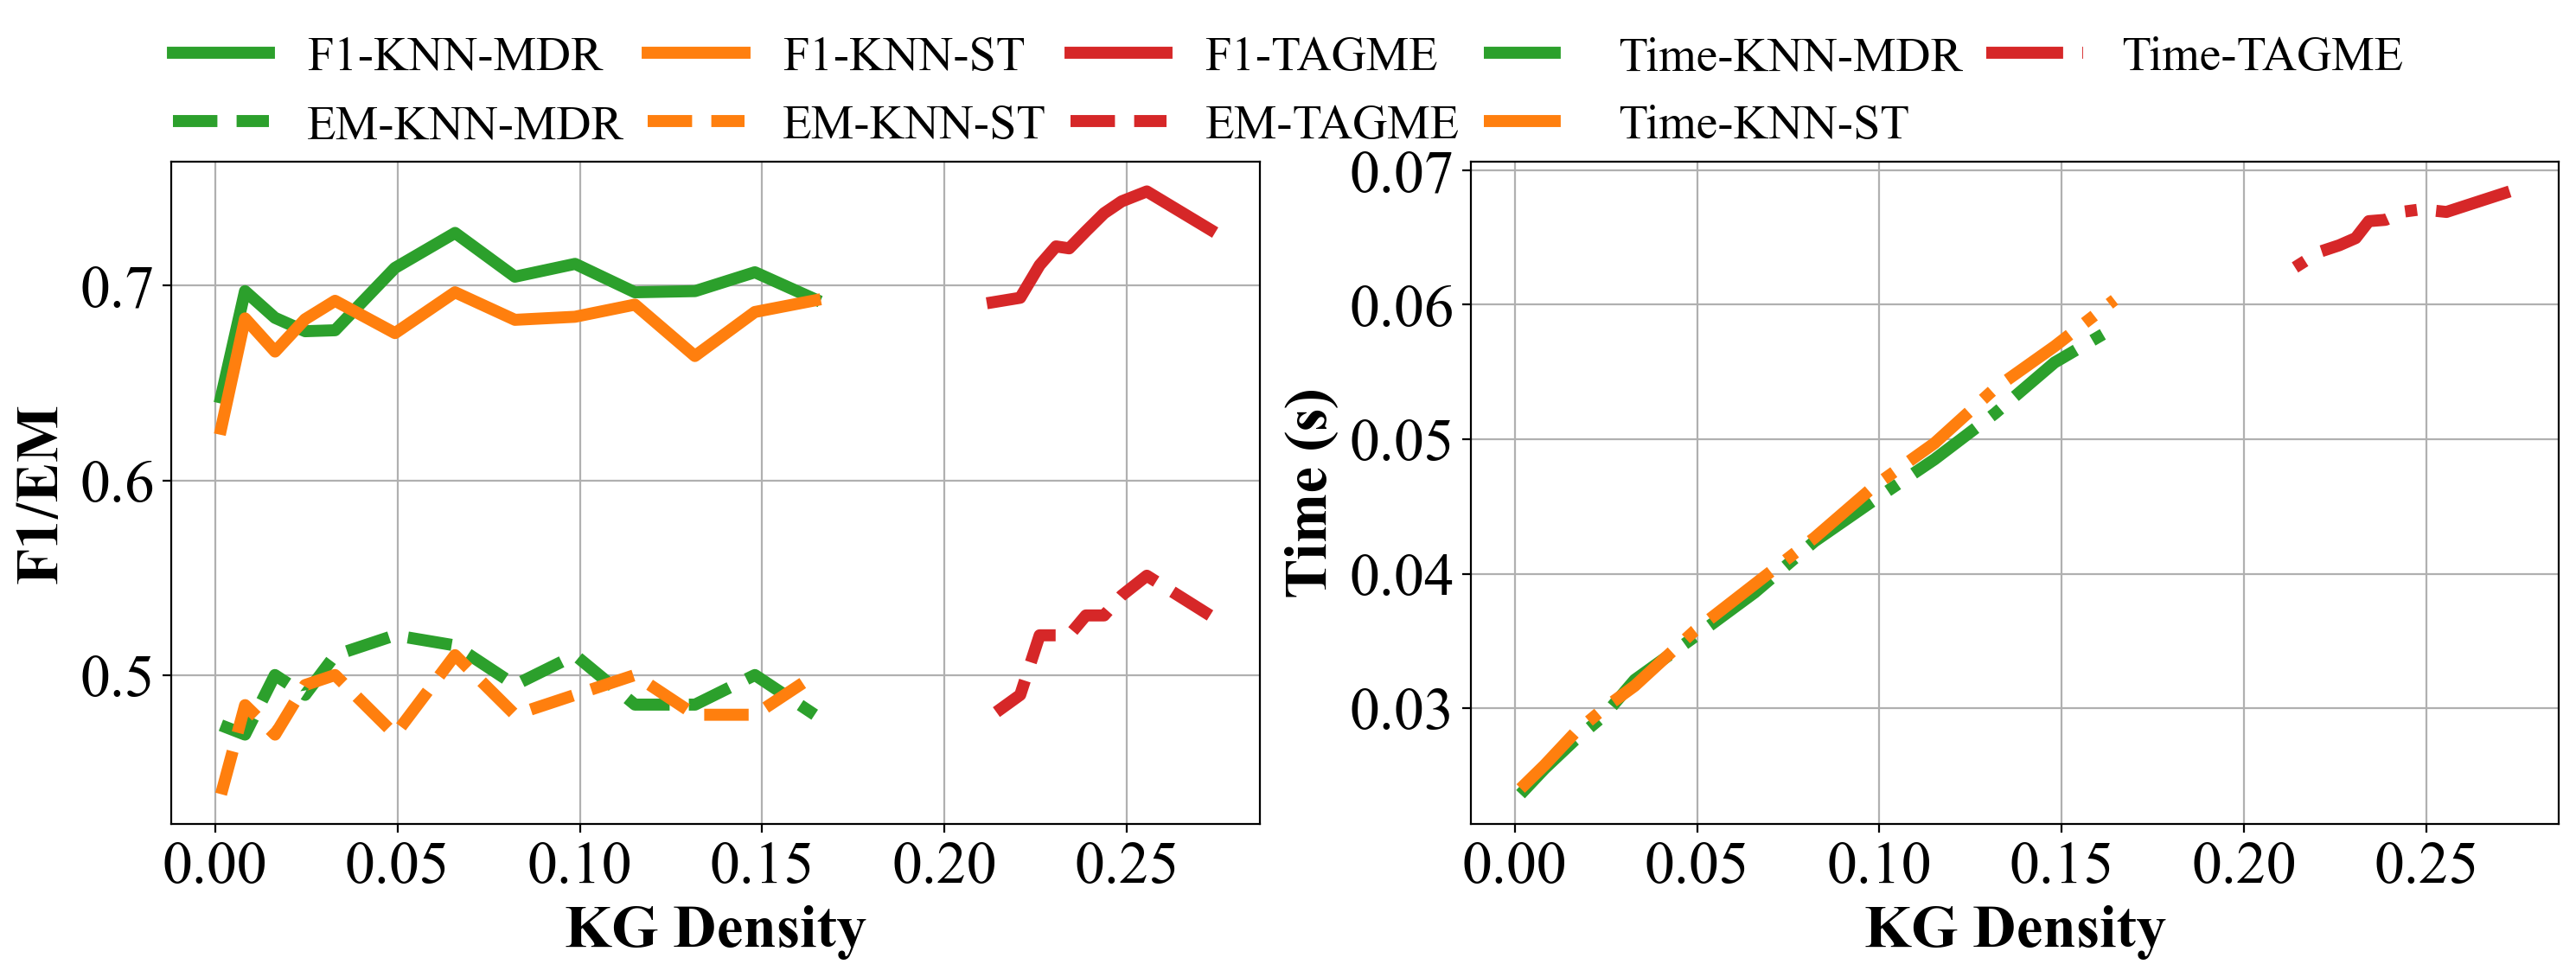
\includegraphics[width=0.48\textwidth]{Figure/combined_graph_hotpotqa.png}
    
    \caption{The performance/latency increases as the KG density increases. The results are averaged across 100 randomly sampled questions on HotpotQA.}
    \label{fig-hotpotqa_graph_perform}
    \vspace{-3ex}
\end{figure}



\subsection{Performance Comparison on MD-QA}\label{sec-performance}
We compare the MD-QA performance of the proposed KGP-T5 and other baselines in Table~\ref{tab-mainperform10}. Firstly, the baselines `None/Golden' achieve the worst/best performance because one provides no context and the other provides the golden context. All other baselines achieve the performance in-between because the retrieved context only covers the partial of the golden supporting facts. Our proposed methods KGP-T5 rank at the Top-1 except for the Golden baseline. The 2$^\text{nd}$-performing baseline MDR fine-tunes a RoBERTa-base encoder by predicting the next supporting fact based on the question and the already retrieved contexts~\cite{xiong2020answering}. This next-passage prediction pretext task equips the model with the reasoning capability of the knowledge across different passages and hence increases the quality of the retrieved contexts. The other deep-learning-based retriever DPR achieves much worse performance than MDR because it only fine-tunes the encoder by maximizing the similarity between the query and its supporting facts regardless of their sequential order, demonstrating the importance of understanding the logical order of different knowledge when solving MD-QA~\cite{xiong2020answering}. By comparing the MD-QA performance across different datasets, we find that all baselines perform better on HotpotQA than on IIRC. This is because questions in HotpotQA are generally simpler than in IIRC. Existing works~\cite{jiang2019avoiding} have shown that some questions in HotpotQA can be easily answered following shortcuts while questions in IIRC sometimes necessitate arithmetic skills to derive answers numerically, e.g., `How many years did the event last when Wingfield lost his fortune?', which poses unique difficulty due to LLMs' inferior arithmetic capability~\cite{yuan2023well}.

Moreover, without any particular design for document structures, no existing baselines can handle structural questions in PDFTriage, e.g. `What is the difference between Page 1 and Page 2' or `In Table 3, which station has the highest average flow rate?'. Fortunately, with the constructed KG incorporating structural nodes and our designed traversal algorithm retrieving structural contexts, our proposed method achieves 67\% Struct-EM.

% \begin{figure}[t!]
%     \centering
%     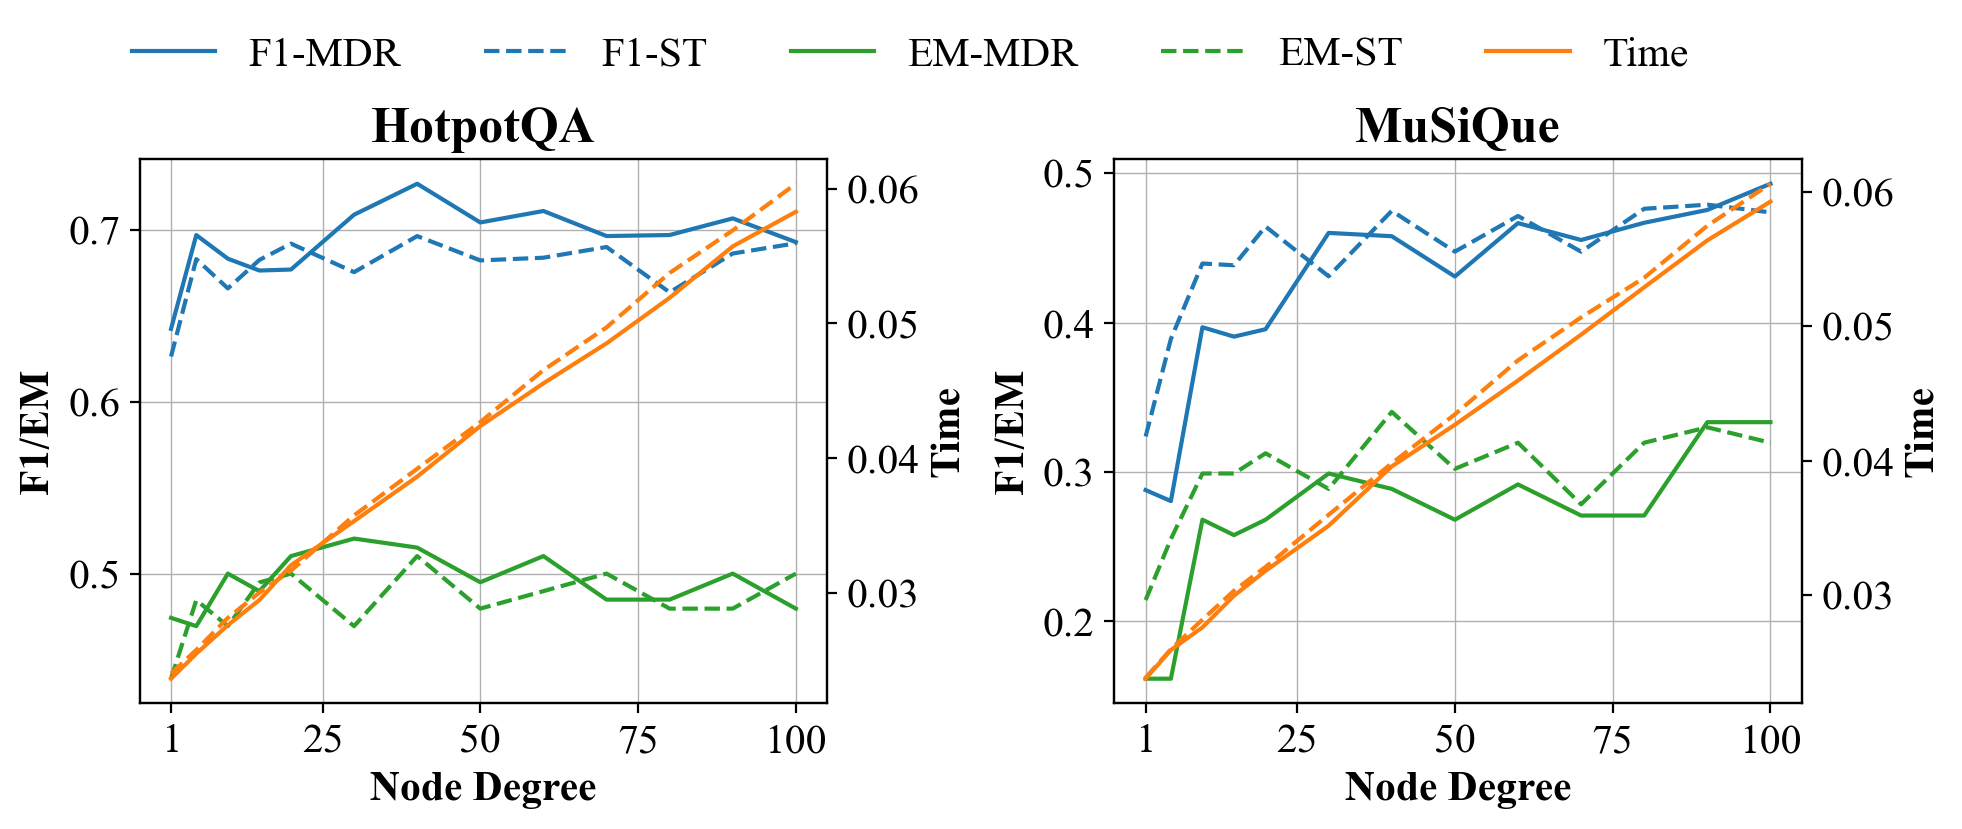
\includegraphics[width=0.5\textwidth]{Figure/Graph_analysis.png}
%     \caption{MD-QA performance first increases and then stays stable as the graph density increases while the search latency also increases. To reduce the time for calling LLMs, we only report the performance on 100 questions from the original 500 questions.}
%     \label{fig-graphimpact}
% \end{figure}



\begin{figure*}[t!]
    \centering
    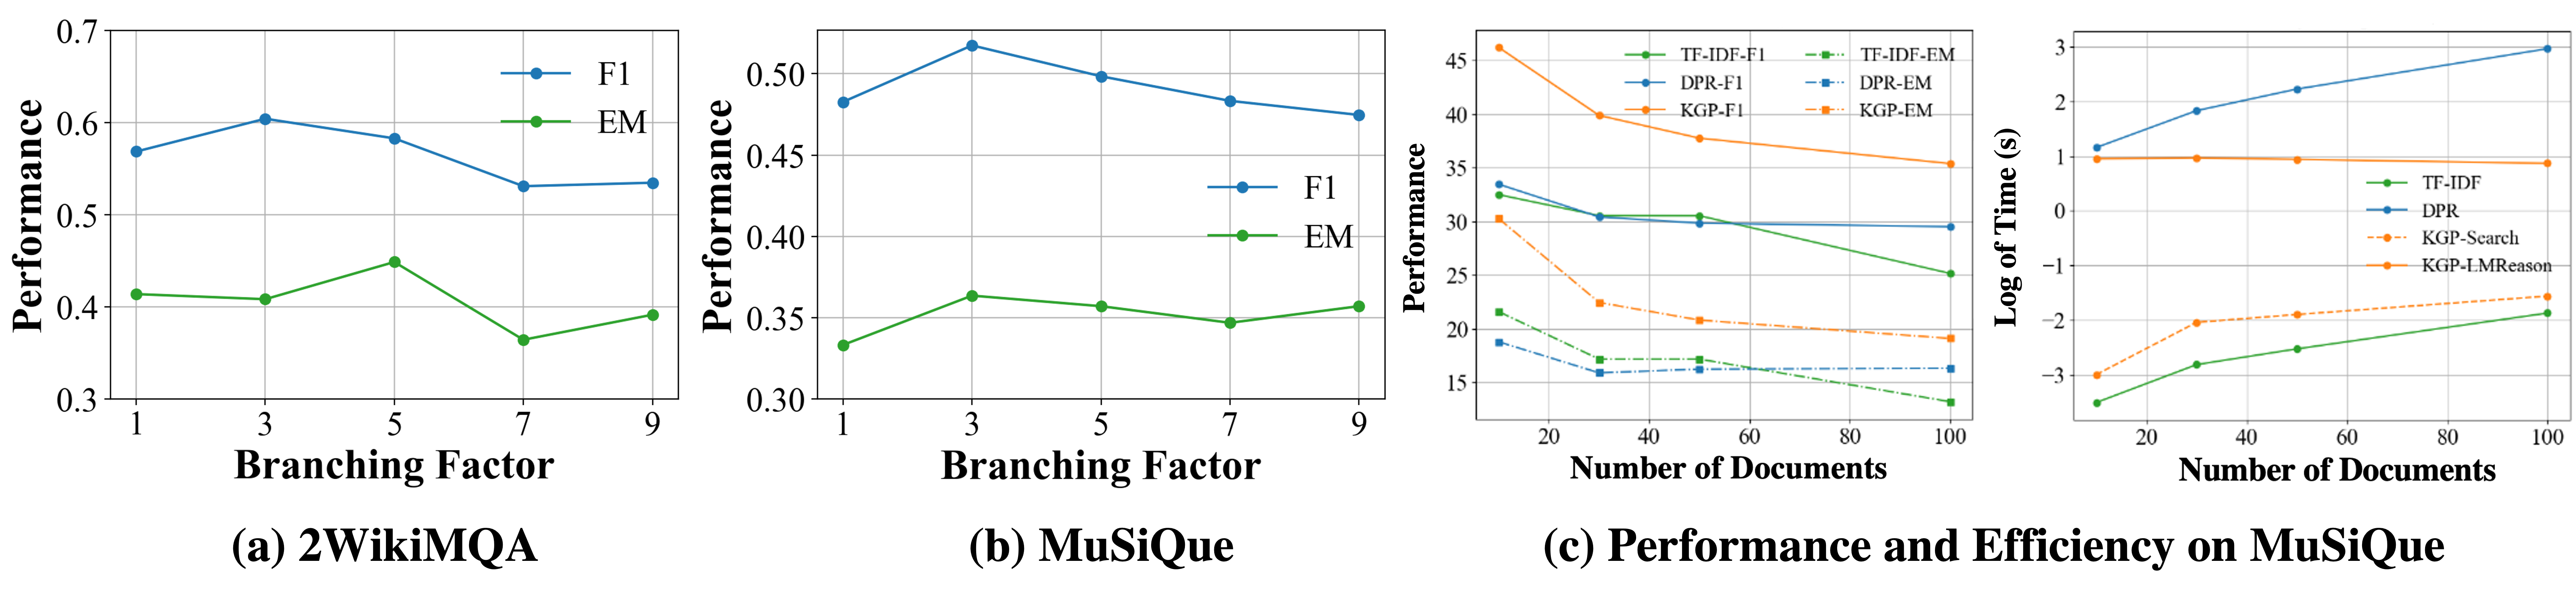
\includegraphics[width=1\textwidth]{Figure/analysis.png}
    \vspace{-5ex}
    \caption{\textbf{(a)-(b)}: Performance first increases and then decreases as the branching factor increases. The results are averaged across 100 sampled questions on 2WikiMQA and MuSiQue. \textbf{(c)}: Performance/Efficiency increases/decreases as the number of documents increases on MuSiQue. KGP-T5 achieves higher performance/efficiency than DPR.}
    \vspace{-2ex}
    \label{fig-analysis}
\end{figure*}




\begin{table}[t!]
\vspace{-2ex}
\tiny
\setlength\tabcolsep{2pt}
\caption{Comparing different LLM-based KG Traversal Agents, including off-the-shelf ChatGPT equipped with few-shot demonstration with fine-tuned LLaMA/T5/MDR on TAGME-constructed KG.}
\begin{tabular}{l|ccc|ccc|ccc|ccc}
\hline
 \textbf{Traversal} & \multicolumn{3}{c|}{\textbf{HotpotQA}} & \multicolumn{3}{c|}{\textbf{IIRC}} & \multicolumn{3}{c|}{\textbf{2WikiMQA}} & \multicolumn{3}{c}{\textbf{MuSiQue}} \\
 \textbf{Agent}  & Acc & EM & F1 & Acc & EM & F1 & Acc & EM & F1 & Acc & EM & F1 \\
\hline
% \rowcolor{grey!15} 
TF-IDF & 73.52 & 43.79 & 63.14  & 46.30  & 27.70  & 41.43  & 58.12  & 35.07 & 45.95 & 44.67 & 21.93 & 32.90\\
\hline
% \rowcolor{orange!15} 
MDR & 75.72 & 46.09 & 65.77 & \textbf{49.58} & \textbf{29.32} & \textbf{43.21} & 60.94 & 37.22 & 51.29 &  \textbf{51.22} & \underline{27.76} & \underline{41.11}\\
\hline
% \rowcolor{purple!15} 
ChatGPT & \textbf{77.80} & 46.03 & \underline{66.57} & 46.27 & 26.01 & 39.35 & 61.62 & 36.16 & 49.39 & 50.61 & 26.92 & 38.66 \\
% \rowcolor{purple!15} 
LLaMA & 75.66 & \underline{46.22} & 66.31 & \underline{49.57} & \underline{28.09} & \underline{42.56} & \underline{62.45} & \underline{37.55} & \underline{52.45} & 50.81 & 26.72 & 40.01 \\
% \rowcolor{purple!15} 
T5 & \underline{76.53} & \textbf{46.51} & \textbf{66.77} & 48.28 & 26.94 & 41.54 & \textbf{63.50} & \textbf{39.80} & \textbf{53.50} & \underline{50.92} & \textbf{27.90} & \textbf{41.19} \\
\hline
\end{tabular}
\label{tab-ablation}
\vspace{-4ex}
\end{table}

\subsection{Impact of the Constructed Graph}\label{sec-graphimpact}
We construct KGs with varying densities by varying the hyperparameters of TF-IDF/KNN-ST/KNN-MDR/TAGME, and studying its impact on the performance and the neighbor matching time of MD-QA using KGP-T5. Since the LLM-based graph traversal agent selects the next node to visit from neighbors of already visited nodes, the chance that it hits the supporting facts increases as neighbors increase. In contrast, the neighbor matching efficiency decreases as the candidate pool, i.e., $\mathcal{N}_j$ in Eq~\eqref{eq-lmtraversal}, increases. As evidenced in Figure~\ref{fig-hotpotqa_graph_perform}, we observe a similar trend, i.e., as KG density increases, the F1/EM increases and stays stable while the latency for selecting the most promising neighbors to visit next also increases. KNN-MDR achieves better performance than KNN-ST when the density of the two constructed KGs is the same. This is because the encoder in KNN-ST is pre-trained on wide-spectrum datasets while the encoder in MDR is specifically pre-trained on the HotpotQA by the pretext task of predicting the next supporting facts. Therefore, the embedding similarity and the corresponding neighbor relations better reflect the logical associations among different passages, which aligns with the better constructed KG by KNN-MDR than KG by KNN-ST in Figure~\ref{fig-hotpotqa_graph}. Compared with KNN-MDR/ST, TAGME delivers superior performance at the cost of increasing latency since the generated KG by TAGME is denser than KGs by KNN-ST/MDR.





\vspace{-1ex}
\subsection{Impact of Graph Traversal Agent}\label{sec-LLMimpact}
Here we study the influence of using different LLM agents to traverse over TAGME-constructed KG on MD-QA. Specifically, we compare agents that select the next neighbor to visit randomly or intelligently via guidance from ChatGPT, LLaMA, T5, and MDR in Table~\ref{tab-ablation}. Because the random agent only blindly traverses the KG without any guidance from LLM, it unavoidably collects irrelevant passages and hence achieves the worst performance than others under LLMs' guidance. This aligns with our previous observation on the low precision in Figure~\ref{fig-hotpotqa_graph} and further demonstrates the necessity of using LLMs to guide the graph traversal. Interestingly, we find that KGP-T5 performs better than LLaMA even though the parameters of LLaMA-7B are more than the ones with T5-0.7B. We hypothesize this is because LLaMA-7B requires more data to fine-tune than T5-0.7B.



\vspace{-1ex}
\subsection{Sensitivity Analysis}\label{sec-sensi}
Here we perform the sensitivity analysis of the branching factor (the number of nodes selected from candidate neighbors to visit next). In Figure~\ref{fig-analysis}(a)-(b), the performance first increases as the branching factor increases because more passage nodes selected from the candidate neighbors lead to more reasoning paths to reach the final answer. However, as we fix the context budget to ensure fair comparison (i.e., the total number of passages we are allowed to retrieve for each question is the same across all baselines), the performance declines as the branching factor increases because the number of initial seeding nodes diminishes, leading to reduced coverage of the KG. Furthermore, we compare the efficiency of KGP when the constructed KG includes different numbers of documents in Figure~\ref{fig-analysis}(c). KGP consistently achieves higher performance than other baselines and higher efficiency than embedding-based DPR. TF-IDF is slightly faster than KGP because it is a purely heuristic-based method. 


